%%%%%%%%%%%%%%%%%%%%%%%%%%%%%%%%%%%%%%%%%
% University/School Laboratory Report
% LaTeX Template
% Version 3.0 (4/2/13)
%
% This template has been downloaded from:
% http://www.LaTeXTemplates.com
%
% Original author:
% Linux and Unix Users Group at Virginia Tech Wiki 
% (https://vtluug.org/wiki/Example_LaTeX_chem_lab_report)
%
% License:
% CC BY-NC-SA 3.0 (http://creativecommons.org/licenses/by-nc-sa/3.0/)
%
%%%%%%%%%%%%%%%%%%%%%%%%%%%%%%%%%%%%%%%%%

%----------------------------------------------------------------------------------------
%	PACKAGES AND DOCUMENT CONFIGURATIONS
%----------------------------------------------------------------------------------------

\documentclass{article}

\usepackage[version=3]{mhchem} % Package for chemical equation typesetting
\usepackage{siunitx} % Provides the \SI{}{} command for typesetting SI units

\usepackage{graphicx}
\usepackage{caption}
\usepackage{subcaption}

\usepackage{float}

\usepackage[T1]{fontenc} % allow small bold caps

\usepackage{listings}
\usepackage{color}

\definecolor{dkgreen}{rgb}{0,0.6,0}
\definecolor{gray}{rgb}{0.5,0.5,0.5}
\definecolor{mauve}{rgb}{0.58,0,0.82}

\lstset{frame=tb,
  language=Python,
  aboveskip=2mm,
  belowskip=2mm,
  showstringspaces=false,
  columns=flexible,
  basicstyle={\small\ttfamily},
  numbers=none,
  numberstyle=\tiny\color{gray},
  keywordstyle=\color{blue},
  commentstyle=\color{dkgreen},
  stringstyle=\color{mauve},
  breaklines=true,
  breakatwhitespace=true
  tabsize=2
}

\setlength\parindent{0pt} % Removes all indentation from paragraphs

\renewcommand{\labelenumi}{\alph{enumi}.} % Make numbering in the enumerate environment by letter rather than number (e.g. section 6)

\usepackage[margin=1in]{geometry}

\usepackage{amssymb}

%\usepackage{times} % Uncomment to use the Times New Roman font

%----------------------------------------------------------------------------------------
%	Title
%----------------------------------------------------------------------------------------

\begin{document}
\pagenumbering{gobble}

\title{6.036: Machine Learning}
\author{
  Ryan Lacey <rlacey@mit.edu>\\
  \footnotesize \texttt{Collaborator(s): Charles Liu, Jorge Perez}
}
        
\maketitle
        

\begin{enumerate}
\item[1.]
	$P_1$-(0.1,0.15)  $P_2$-(0.3,0.15) $P_3$-(0.12,0.17) $P_4$-(0.3,0.17) $P_5$-(0.2,0.18) $P_6$-(0.22,0.19) $P_7$-(0.45,0.2)\\

	$h = (-x_2 + (0.17-\epsilon))$\\

	$\mathcal{E} = 2(\frac{1}{7}) = \frac{2}{7}$\\
	
	$\alpha = \frac{1}{2} \log \left(\frac{5/7}{2/7}\right) = \frac{1}{2} \log \left(\frac{5}{2}\right)$\\
	
	$w_1=w_2=w_4=w_6=w_7=\frac{1}{7}e^{-\frac{1}{2} \log \left(\frac{5}{2}\right)}$\\
	$w_3=w_5=\frac{1}{7}e^{\frac{1}{2} \log \left(\frac{5}{2}\right)}$\\	
	
	$\displaystyle\sum_{w_i \in W}{w_i} = \frac{2\sqrt{10}}{7} \therefore C=\frac{7}{2\sqrt{10}}$\\
	
	New weights\\
	$w_1=w_2=w_4=w_6=w_7=\frac{1}{10} $\\
	$w_3=w_5=\frac{1}{4}$\\

\newpage

\item[2.]
		$h_1 = (-x_1 + 0.21)$ \hfill $\mathcal{E}_1 = \frac{1}{7}$ \hfill $\alpha_1 = \frac{1}{2} \log \left(6\right) = 0.895$\\
		
		$w_1=w_3=w_4=w_5=w_6=w_7=\frac{1}{7}e^{-\frac{1}{2} \log \left(6\right)}$\\
		$w_2=\frac{1}{7}e^{\frac{1}{2} \log \left(6\right)}$\\	
		
		$\displaystyle\sum_{w_i \in W}{w_i} = \frac{2\sqrt{6}}{7} \therefore C=\frac{7}{2\sqrt{6}}$\\
		
		New weights\\
		$w_1=w_3=w_4=w_5=w_6=w_7=\frac{1}{12} $\\
		$w_2=\frac{1}{2}$\\
		\makebox[\linewidth]{\rule{\textwidth}{0.4pt}}
		$h_2 = (-x_2 + 0.185)$ \hfill $\mathcal{E}_2 = \frac{1}{12}$ \hfill $\alpha_2 = \frac{1}{2} \log \left(11\right) = 1.19$\\
		
		$w_1=w_3=w_5=w_6=w_7=\frac{1}{12}e^{-\frac{1}{2} \log \left(11\right)}$\\
		$w_2=\frac{1}{2}e^{-\frac{1}{2} \log \left(11\right)}$\\
		$w_4=\frac{1}{12}e^{\frac{1}{2} \log \left(11\right)}$\\
		
		$\displaystyle\sum_{w_i \in W}{w_i} = \frac{\sqrt{11}}{6} \therefore C=\frac{6}{\sqrt{11}}$\\
		
		New weights\\
		$w_1=w_3=w_5=w_6=w_7=\frac{1}{22} $\\
		$w_2=\frac{3}{11}$\\
		$w_4=\frac{1}{2}$\\
		\makebox[\linewidth]{\rule{\textwidth}{0.4pt}}
		$h_3 = (-x_2 + 0.16)$ \hfill $\mathcal{E}_3 = \frac{1}{11}$ \hfill $\alpha_3 = \frac{1}{2} \log \left(10\right) = 1.15$\\
		
		$w_1=w_6=w_7=\frac{1}{22}e^{-\frac{1}{2} \log \left(10\right)}$\\
		$w_2=\frac{3}{11}e^{-\frac{1}{2} \log \left(10\right)}$\\
		$w_3=w_5=\frac{1}{22}e^{\frac{1}{2} \log \left(10\right)}$\\
		$w_4=\frac{1}{2}e^{-\frac{1}{2} \log \left(10\right)}$\\
		
		$\displaystyle\sum_{w_i \in W}{w_i} = \frac{2\sqrt{10}}{11} \therefore C=\frac{11}{2\sqrt{10}}$\\
		
		New weights\\
		$w_1=w_6=w_7=\frac{1}{40} $\\
		$w_2=\frac{3}{20}$\\
		$w_3=w_5=\frac{1}{4}$\\
		$w_4=\frac{11}{40}$\\
		\makebox[\linewidth]{\rule{\textwidth}{0.4pt}}
		$w_1=w_6=w_7=\frac{1}{2\sqrt{165}}$ \hfill $w_2=\sqrt{\frac{3}{55}}$ \hfill  $w_4=0.5\sqrt{\frac{11}{15}}$ \hfill  $w_3=w_5=\sqrt{\frac{5}{33}}$ \\
		
		Loss sum = 1.556\\

\newpage

\item[3.]
	Yes, it is advantageous to pick the classifier that minimizes exponential loss because one can expect such a classifier to generalize better on test data. Additionally, the boosting algorithm is resistant to overfitting because "the complexity of the ensemble does not increase very quickly as a function of the number of base learners". Thus we would not worry about using additional stumps in the ensemble in a way similar to concerns of overfitting a classifier by increasing the order of the classifying polynomial.

\bigskip

\item[4.]
	 $P(h_i \text{ correctly classifies random point}) = |1 - \frac{\phi}{\pi} | = | 1 - \frac{i}{100} | $

\bigskip

\item[5.]
	 Number of classifiers given by area portion of disk classifiers contain.\\
	 \medskip\\
	 $\mathcal{H}_\frac{1}{10}$ covers $\frac{9}{10}$ of the area in the range $[\frac{-9\pi}{10}, \frac{9\pi}{10}]$\\

	 With stepsize of $\frac{\pi}{100}$ we obtain 181 classifiers\\
	 \bigskip\\
	 $\mathcal{H}_\frac{1}{5}$ covers $\frac{4}{5}$ of the area in the range $[\frac{-4\pi}{5}, \frac{4\pi}{5}]$\\

	 With stepsize of $\frac{\pi}{100}$ we obtain 161 classifiers\\

\newpage

\item[6.]
	$P(\text{5 correctly classified points}) = 2 \times\frac{1}{200} \displaystyle\sum_{i=1}^{99}{\left(1 - \frac{\phi}{\pi}\right)^5 + \frac{1}{200}}  = \frac{1}{100} \displaystyle\sum_{i=1}^{99}{\left(1 - \frac{i}{100}\right)^5 + \frac{1}{200}} = 0.1667$\\
	 Symmetry of probabilities across opposite ends of circle allows us to add up probabilities on one half, then double it.\\
	 Point 100 has probability zero, so we can remove if from our summation.\\
	 Point 200 has probability one, but should only be included once, so we add the probability of $h_{200}$ after the summation.\\ 
	 \bigskip\\
	 \bigskip\\
	 \bigskip\\	
	 $P(h \in  \mathcal{H}_\frac{1}{10} \text{ | 5 correctly classified points} ) = \dfrac{P(\text{5 correctly classified points | } h \in  \mathcal{H}_\frac{1}{10} )P(h \in  \mathcal{H}_\frac{1}{10})}{P(\text{5 correctly classified points})}$\\
	 \medskip\\
	 $P(h \in  \mathcal{H}_\frac{1}{10}) = \frac{181}{200} = 0.905$ from \texttt{(5)}.\\
	 \medskip\\
	 $P(\text{5 correctly classified points | } h \in  \mathcal{H}_\frac{1}{10})  = \frac{1}{181}{\displaystyle\sum_{i=10}^{190}{\left|1 - \frac{i}{100}\right|^5}} = 0.101$\\
	 \medskip\\
	 $\therefore P(h \in  \mathcal{H}_\frac{1}{10} \text{ | 5 correctly classified points} ) = \frac{(0.101)(0.905)}{0.1667}  = 0.548$\\
	 \bigskip\\
	 \bigskip\\
	 \bigskip\\	 
	 $P(h \in  \mathcal{H}_\frac{1}{5} \text{ | 5 correctly classified points} ) = \dfrac{P(\text{5 correctly classified points | } h \in  \mathcal{H}_\frac{1}{5} )P(h \in  \mathcal{H}_\frac{1}{5})}{P(\text{5 correctly classified points})}$\\
	\medskip\\
	$P(h \in  \mathcal{H}_\frac{1}{5}) = \frac{161}{200} = 0.805$ from \texttt{(5)}.\\
	\medskip\\
	$P(\text{5 correctly classified points | } h \in  \mathcal{H}_\frac{1}{5})  = \frac{1}{161}{\displaystyle\sum_{i=20}^{180}{\left|1 - \frac{i}{100}\right|^5}} = 0.0563$\\
	\medskip\\
	$\therefore P(h \in  \mathcal{H}_\frac{1}{5} \text{ | 5 correctly classified points} ) = \frac{(0.0563)(0.805)}{0.1667}  = 0.272$\\

\bigskip

\item[7.]
	Generalization error $= \dfrac{\log (|H|) + \log (\frac{1}{\delta})}{n}$\\

	$0.1 = \dfrac{\log (200) + \log (\frac{1}{1 - 0.995})}{n} \implies n = \dfrac{\log (200) + \log (\frac{1}{0.005})}{0.1} = 105.96$\\

	We cannot have fractional points classified correctly, so we estimate 106 training points would be correctly classified.
	
\newpage

\item[8.]	
	The VC diension of a stump in two-dimensional space is 3. Below is an example shattering three points for all possible labelings.\\
	\bigskip\\
	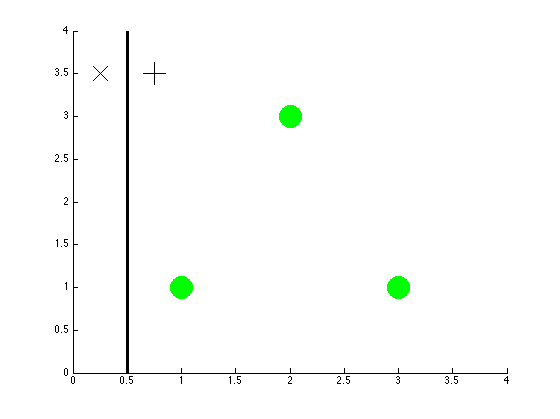
\includegraphics[scale=0.25]{../images/ggg} \hfill 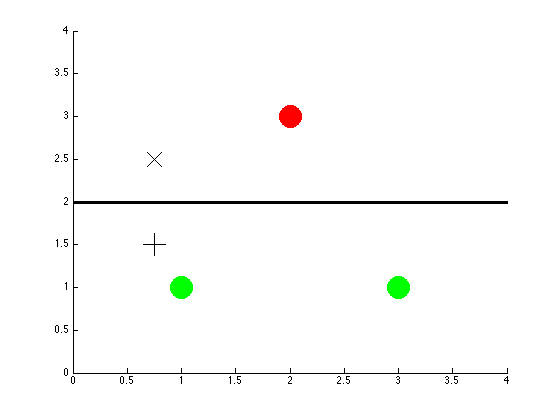
\includegraphics[scale=0.25]{../images/ggr}\\
	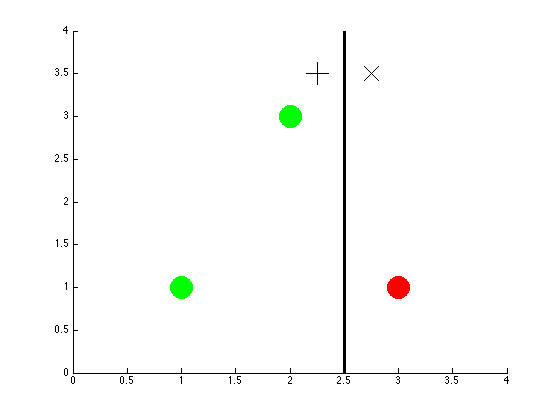
\includegraphics[scale=0.25]{../images/grg} \hfill 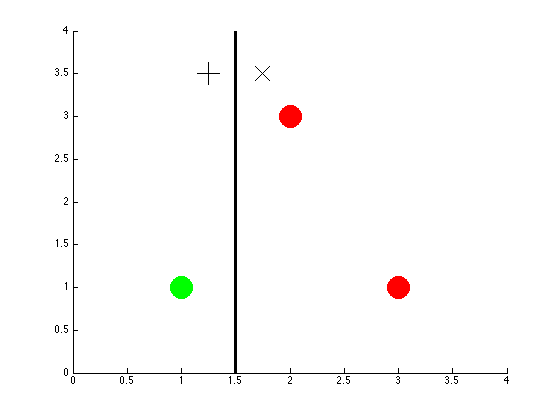
\includegraphics[scale=0.25]{../images/grr}\\
	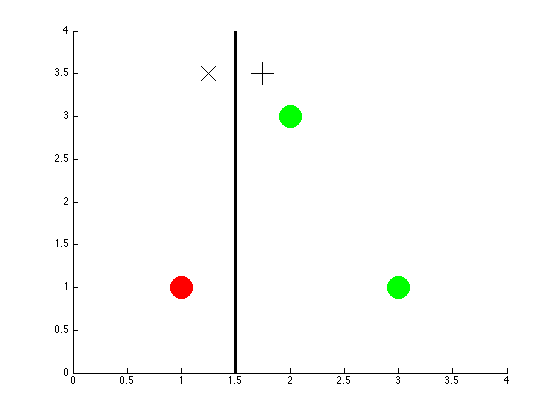
\includegraphics[scale=0.25]{../images/rgg} \hfill 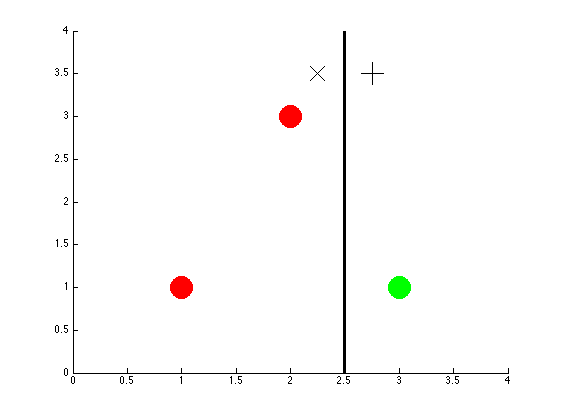
\includegraphics[scale=0.25]{../images/rgr}\\
	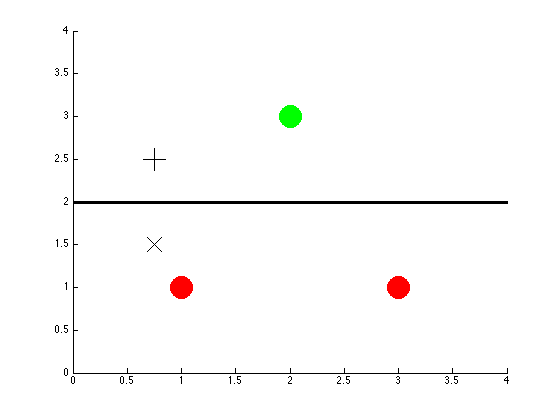
\includegraphics[scale=0.25]{../images/rrg} \hfill 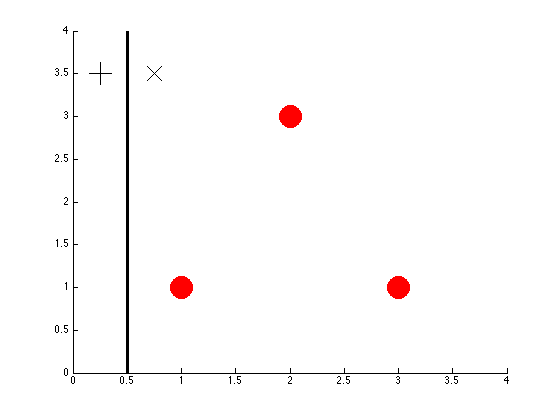
\includegraphics[scale=0.25]{../images/rrr}\\
	\bigskip\\
	A single stump cannot shatter four points, however. If all four points were colinear, then one could alternate the labels in the line of points \texttt{+ - + -}. Similarly, if three points were colinear one could alternate labels of points \texttt{+ - +}. Without loss of generality consider the points all along the x-axis. No vertical stump could correctly classify all of these points. The location of the fourth point with the three colinear points is irrelevant. Finally we could have the points in some other arrangement. One can draw a line between two pairs of the points so that a \texttt{X} is formed by the lines. If the points connected by lines are labeled the same and the points at the ends of the other line are labeled oppositely then one could not use a stump to classify the points. A case of this was seen in lecture with four points arranged in a square, with each point being the opposite label of its two nearest neighbors and of the same label as the point diagonal from itself.

\newpage

\item[9.]	
	The VC-dimension of a stump can be different in higher dimensions. As an example consider four points in a 16-dimensional space. The features for the four points will looks something like\\
	
	(+1, +1, +1, +1..)\\
	(+1, -1, +1, +1...)\\
	(+1, -1, -1, -1...)\\
	(+1, -1, -1, +1...)\\
	
	Given any labeling of the points, one can then choose a stump that aligns with the column that corresponds with the label. For example if all the points were labeled positive, then one would place the stump along the first dimension. If the first point were positive and the others negative, then one would place the stump along the second dimension. There are $2^{4} = 16$ possible assignments of labels to the points. Therfore we require 16 dimensions so that we can place the stump along the dimension that is represented by the labeling. Since this handles all possible labeling for four points, the single stump can shatter them, meaning the VC-dimension is greater than in the 2D case. To generalize this, we claim that $\log_2(n)$ is that maximum dimensions required to shatter $n$ points.

\end{enumerate}

\end{document}